\chapter{CHOIX DES OUTILS}
\section{CHOIX D'UN OUTIL BI}
Avant de mettre en place un système décisionnel en général le besoin née d’un ensemble de question que se pose le DSI. A chacune de ces questions correspond une réponse venant d’une partie ou un processus du BI. La figure suivant résume cette question que tentent de répondre tout système décisionnel.

\begin{figure}[!htbp]
	\begin{center}
		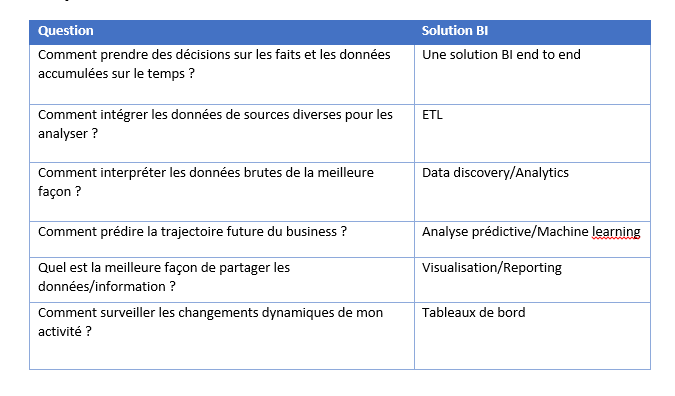
\includegraphics[scale=0.95]{images/tab_question_bi.png}
		\caption{Problèmes et outils BI réponses.}
		\label{use_bi_tools}
	\end{center}
\end{figure}

\subsection{Le choix d’un fournisseur}

Dans le marché de produits BI il existe  plusieurs critères de classement de fournisseurs. Nous les avons segmenté un deux grand groups (Les grands Fournisseur et les plus petit et nouveau fournisseurs).

\begin{figure}[!htbp]
	\begin{center}
		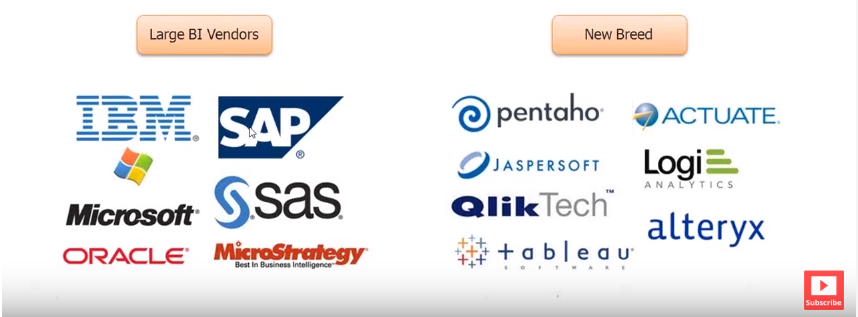
\includegraphics[scale=0.75]{images/compare_bi_vendors.png}
		\caption{Regroupement des fournisseurs de solutions BI}
		\label{use_bi_tools}
	\end{center}
\end{figure}

Toutefois il existe un grand nombre de fournisseur qui offrent des outils spécifique pour des processus BI précis. On a par exemple : 
\begin{list}{•}{ }
   \item INFORMATICA : Pour l’intégration de données (ETL)
   \item RAPIDMINER : Pour l’analyse de données (Analytics)
   \item TALEND : Pour l’intégration de données (ETL)\\
\end{list}

L’un des facteurs qui a motivé notre choix dans ce cas est que PENTAHO s’interface facilement avec la majorité de ces solution qui traitent un seul processus BI. Le tableau de la figure 4.2 fait un récapitulatif de quelques solutions BI qui nous ont semblés pertinentes.\\

\begin{figure}[!htbp]
	\begin{center}
		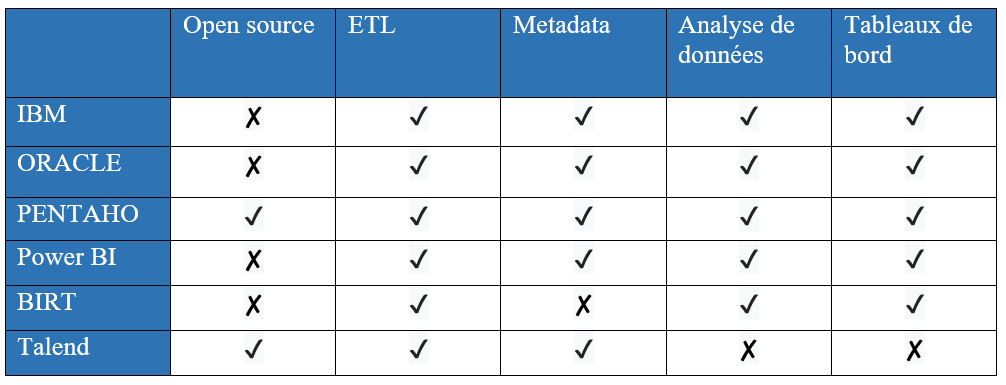
\includegraphics[scale=0.55]{images/compare_bi_vendors_2.png}
		\caption{La suite Pentaho.}
		\label{bi_tools_compare}
	\end{center}
\end{figure}


\subsection{LES ENJEUX D’UN BON CHOIX}

	Avec les solutions de BI qui existent déjà on fait face à un ensemble de difficulté qui ce pendant rendent le choix selon le contexte plus facile. Ces barrières sont les suivantes.
	\begin{list}{•}{ }
	   \item Cout d’installation : La solution des grands fournisseurs ont un cout en infrastructure souvent très élevé car la mise en œuvre des serveurs et des architectures réseau extrêmement couteuses à  mettre en place.
	   \item Cout des licences : Les licences d’exploitation ont un cout assez élevé comparé aux plus petits fournisseurs.
	   \item Temps d’intégration et d’apprentissage long : Les solutions les plus élaboré en matière de BI ont une courbe d’apprentissage plus difficile et l’installation prend plus de temps que les solutions des petits fournisseurs.
	   \item Cout de maintenance élevé : L’augmentation du cout de maintenance est dû au fait que il faut une main d’œuvre qualifié et de qualité parfois pour effectuer même les taches les plus dérisoires.\\
	\end{list}
	
\subsection{LE CHOIX FINAL}

Le plus difficile dans les plus petits et nouveaux fournisseur est le fait de ne pas trouver facilement un logiciel qui gère l’ensemble des processus BI. Cette difficulté nous a fait converger vers un outil en particulier qui n’avait pas ce défaut. Notre choix ces porté sur PENTAHO pour les raison suivantes:
\begin{list}{•}{ }
   \item PENTAHO est une solution tout en un pour tous problèmes d’analyse de données.
   \item Le cout de la licence est abordable et il existe une version community qui est presque gratuit.
   \item Il se superpose facilement sur des solutions partielles et même des grands fournisseurs pour l’analyse ou l’exploitation des données issues de celles-ci.
   \item Il bénéficie d’une grande communauté car il est open source.
   \item Il est facile à faire évoluer et adapter aux besoins grandissent des entreprises (en anglais Scalability)
   \item Les composantes de Pentaho sont des projets libre individuels (Standalone) qui bénéficient chacun d’une forte communauté.\\
\end{list}

Tels sont les point qui ont confortés le choix de Pentaho en tant que solution a notre problématique. La figure suivante est un une correspondance entre d’une part les outils que offre Pentaho et le processus BI qu’il gère.

\begin{figure}[!htbp]
	\begin{center}
		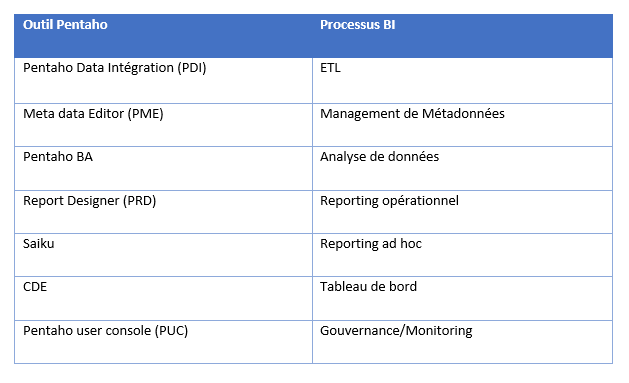
\includegraphics[scale=0.95]{images/tab_pentaho_tools.png}
		\caption{La suite Pentaho.}
		\label{use_bi_tools}
	\end{center}
\end{figure}


\cleardoublepage
\section{CHOIX DU SGBD}

En termes de système de gestion de base de données notre choix s’est porté sur Postgresql car de par son atout majeur d’être très sécurisé il offre les avantages suivants :  
\begin{list}{•}{ }
   \item Au niveau de l’architecture : Postgresql est un système de gestion de base de données de modèle relationnel \& objet.
   \item Au niveau des fonctionnalités : Postgresql facilite la tâche des développeurs dans sa configuration et supporte plus de fonctionnalités tel que CTE (Common Table Expressions), GiST/GIN ou bien les fonctions de fenêtrage par rapport à MySQL qui hélas à du retard.
   \item Au niveau des migrations vers d’autres types de BDD : Il est plus simple de migrer et changer sur d’autres bases de données avec Postgresql. De même pour sauvegarder et restaurer des backups.
 \item Au niveau de la documentation : Postgresql est en forte expansion et sa documentation reste plus claire.
\end{list}

\section{AUTRES OUTILS}
\textbf{LARAVEL }: Laravel est un framework web open-source écrit en \textbf{PHP} respectant le principe modèle-vue-contrôleur et entièrement développé en programmation orientée objet. Laravel est distribué sous licence MIT, avec ses sources hébergées sur GitHub. Ce framework a été utilisé dans le développement de la partie administration de Hosteline. Nous avons développé des routines pour remplir notre Data Warehouse sur cette plateforme.\\

\textbf{Angular} (communément appelé "Angular 2+" ou "Angular v2 et plus") est un cadriciel (framework) coté client open source basé sur \textbf{TypeScript} dirigée par l'équipe du projet Angular à Google et par une communauté de particuliers et de sociétés. Angular est une réécriture complète de \textbf{AngularJS}, cadriciel construit par la même équipe. La partie client de la plateforme est développé sur ce cadriciel. Sur le profile du client a été développé un tableau de bord selon les besoins spécifiés au début de notre etude.\\
